% !TeX root = ../russian-vocab-2021-22.tex

\chapter{Новости}

\section{Ее можно считать жертвой}
\textit{Никита Абрамов, Наталья Гранина}\\
\url{https://lenta.ru/articles/2021/12/22/kinder/}

\textit{Отец девятилетней студентки МГУ \explainDetail{нап\'{а}л}{нападать/напасть}{attack} на людей в вузе. Что о семье Тепляковых думают педагоги?}

У девочки-вундеркинда Алисы Тепляковой, которая в восемь лет \explain{сдала ЕГЭ}{сдавать/сдать экзамен} и поступила на платное отделение психфака МГУ, началась первая сессия. Во вторник, 21 декабря, появилось видео, где ее отец Евгений Тепляков пытается прорваться через пост охраны факультета с криками, что он «хочет поговорить с преподавателями». Администрация факультета вынуждена была прятать их от агрессивного родителя. Еще в сентябре, когда стало известно, что Алиса станет студенткой МГУ, «Лента.ру» попросила прокомментировать это событие известных педагогов. Все они сомневались, что для психики маленького ребенка учеба в вузе будет \explainDetail{посильной}{посильный/-ая}{Within one's strength, abilities, powers (for a task); посильная задача} задачей. Возможно, \explainDetail{опасения}{опасение}{fear} начинают \explainDetail{сбываться}{сбываться/сбыться}{to come true}. Мы публикуем их мнения об Алисе и методах ее отца.

\subsection{Будет не столько студенткой, сколько подопытным объектом}
\textit{Леонид Кацва, автор учебников и пособий по истории России. Преподаватель московской школы № 1543}

Я смотрел видеоинтервью с Алисой Тепляковой. У нее, видимо, очень тренированная \explainDetail{память}{память (ж)}{memory}. Каких-то других качеств она не показала в выступлении. Разговаривает она как семилетка, уровень ее понимания ситуации --- типичный для маленького ребенка. У нас в школе на \explain{педсовете}{teachers' council} перед началом учебного года говорили об этом, многие считают, что вся эта история очень дурно пахнет. \explainDetail{Имеется в виду}{имеется в виду}{it means} не то что девочка сдала ЕГЭ --- \explain{вызубрить}{memorise} какие-то вещи по нескольким предметам на минимальный балл она могла, если у нее действительно вот такая память. Я видел, как она читает --- быстро, но \explain{судя}{judging} по всему общего \explainDetail{смысла}{смысл}{meaning} текста не понимает. Папа \explain{дрессировал}{trained} детей именно на скорочтение. А скорочтение --- это немного не про чтение в том смысле, как мы его понимаем.

У меня нет вопросов к папе. Он хочет доказать некую идею --- что можно в школе не учиться 11 лет, а \explainDetail{освоить}{осваивать/освоить}{to master} все за три года. К девочке у меня тоже вопросов нет. Потому что в данном случае она --- \explain{орудие}{tool} в руках папы, \explain{в какой-то мере}{to an extent} ее даже можно считать жертвой.

У меня есть вопрос к МГУ: \explainDetail{принять}{принимать/принять}{accept} девятилетнего ребенка на психфак --- это надо все же сильно постараться.  Но гораздо больше у меня вопросов к школе,  которая ее  выпустила. Я ничего про эту школу не знаю. Даже не знаю номера. Видимо, она была на домашней форме   \explainDetail{обучения}{обучение}{learning; education}, на уроки не ходила. Не знаю, как это было оформлено --- экстернат или домашнее обучение, этого не могу сказать. Но если она в восемь лет сдала экзамены за все годы обучения, то, \explain{грубо говоря}{roughly speaking}, девочка должна была с шести лет сдавать экзамены каждые два-три месяца. Это если их принимали.

Папа говорит совершенно открыто, что девочка не прочитала ни одного программного литературного произведения, что она знакомилась с художественными книгами в виде кратких пересказов. Я понимаю, что так некоторые дети и делают, даже в 17-летнем возрасте. Но \explain{все-таки}{even so} это принято скрывать, а не превращать в манифест.

Я 40 лет преподаю историю и, как говорится, зуб даю, что если ребенка начать спрашивать не на уровне тестов, кто командовал теми-то войсками, кто был генеральным секретарем тогда-то, министром, великим князем тогда-то, а начать спрашивать \explain{всерьёз}{seriously}, с причинно-следственными связями, с характеристиками событий, то не о чем будет говорить. Специалисты по естественным наукам и физике также замечают, что даже на уровне физиологии не может ребенок в таком возрасте эти дисциплины качественно осваивать.

У нас были вундеркинды. И я знаю случаи, когда в вуз приходил учиться 14-летний студент. Однако разница между 14 и 17 годами, когда \explain{пол\'{о}жено}{one should, one ought to, one is supposed to} сдавать ЕГЭ, \explain{на порядок}{by an order of magnitude} меньше.
Я уж не говорю о разнице между 17 годами и девятью. Поэтому я в данном случае вижу какую-то \explain{недобросовестность}{dishonesty} с разных сторон. И прежде всего --- школы.
Возможно, она просто решила \explain{подыграть}{play along} папе, не знаю почему. Либо просто отвязаться от этого папы. Потому что папа такой, что проще согласиться на его \explainDetail{условия}{условие}{condition; term}, чем объяснять ему, почему этого делать не стоит.
Но, с другой стороны, есть и контраргумент, почему это может быть не так. За Алисой --- на подходе очередь из ее братьев и сестер. \explainDetail{Причём}{причём}{moreover} если у Алисы имя обычное --- среди девочек школьного возраста Алисы встречаются, то у остальных детей в семье имена скандинавских богов, а не детей из России. И тут у меня \explain{ощущение}{sensation}, что психологическое состояние папы от старшего ребенка к младшим начало \explainDetail{усугубляться}{усугубляться/усугубиться}{get worse}.

На мой взгляд, тут широкое поле деятельности для \explain{Рособрнадзора}{Федеральная служба по надзору в сфере образования и науки (Рособрнадзор): Federal Service for Supervision in Education and Science}. Не думаю, что тут речь о \explainDetail{мошенничестве}{мошенничество}{fraud; cheating} при ЕГЭ --- ребенок с натренированной памятью мог рассчитывать на минимальные баллы, чтобы экзамен считался сданным. Но \explain{полноценное}{of full value} среднее образование она получить не могла. Девочка под папиным \explainDetail{внушением}{внушение}{suggestion} говорит: в школе 11 лет учатся, а в институте --- пять, значит, институт --- проще, я его окончу за два года. Эти слова ребенка \explain{цитируют}{quote} \explain{СМИ}{средства м\'{а}ссовой информации}. Предположим, она окончит институт в 11 лет. Вы пойдете на консультацию к такому специалисту-психологу? Я, честно говоря, \explainDetail{остерегусь}{остерегаться/остеречься}{beware}.

\begin{fancyquotes}
    Это моя гипотеза --- и кроме догадок она ни на чем не основана, --- что на психфак ее приняли не столько для того, чтобы обучать как полноценного студента, сколько для того, чтобы ставить своего рода эксперимент. То есть в этой ситуации она будет не столько студенткой, сколько подопытным объектом, потому что с точки зрения психологии в ее развитии есть какие-то аномалии --- скорее всего положительные, а может быть, и не только
\end{fancyquotes}

Папа говорит, что учител\'{я}, которые заставляют свободно читающего ребенка \explain{по слог\'{а}м}{syllable by syllable} \explainDetail{произносить}{произносить/произнести}{pronounce; (present tense) произнош\'{у}, произн\'{о}сишь, произн\'{о}сят} ма-ма мы-ла ра-му, --- преступники. У него все --- преступники, один он --- молодец. Совершенно понятно, что папа преследует какие-то цели. Не могу сказать, что они материальные, \explain{по-в\'{и}димому}{apparently}, он хочет \explainDetail{прославиться}{прославляться/прославиться}{become famous}, стать великим реформатором образования или кем-то еще \explain{в этом роде}{like that}. Но мне кажется, что эти эксперименты очень опасные.

В моей практике были дети, которые перескакивали через класс --- из шестого в восьмой, из восьмого в десятый. Таких случаев у меня было, если не ошибаюсь, три. Эти ситуации на состояние детей оказали скорее \explain{отрицательное влияние}{negative influence}, чем положительное. Ребята были развитые, скучали в классах по возрасту, но когда их перевели на год вперед, они совершенно потерялись. Мне кажется,  что так делать не надо.

У меня есть дети, которые очень одарены математически и учатся в математическом классе. Они становились призерами Всероссийских олимпиад, но это не повод считать, что во всем остальном дети так же одарены. Знаете, как говорил великий русский поэт Козьма Прутков: «Специалист подобен флюсу, полнота его односторонняя». \explainDetail{Допускаю}{допуск\'{а}ть/допуст\'{и}ть}{admit}, что талантливые дети могут оканчивать школу, \explain{допустим}{let's say}, не за 11 лет, а за девять. Но в то, что ребенок может окончить школу в 9 лет, --- не верю.

\subsection{Слишком умных учеников частенько боятся}
\textit{Леонид Перлов, почетный работник общего образования России, много лет преподавал географию в одной из лучших математических школ страны Лицей «Вторая школа»}

В обычных школах слишком умных учеников частенько просто боятся. Потому что учитель --- живой человек. Он понимает, когда у него не получается, и не понимает --- почему. А не получается просто потому, что он раньше мог не иметь дела с такими детьми. Или школьная администрация от него требует одно, а ребенку нужно совершенно другое. И как найти в этом приемлемую середину --- очень сложный вопрос.

С такими ребятами действительно трудно, \explain{ничуть}{not at all} не легче, чем с детьми с аутическим компонентом, с другими \explainDetail{особенностями}{особенность}{feature, singularity, characteristic, particulatiry} развития.

Просто здесь трудности другого рода. Учитель должен очень много знать не только в области своей математики, географии или литературы, а именно в области педагогики. Эти дети больше требуют, они иначе \explain{воспринимают}{perceive} действительность, спос\'{о}бны быстро анализировать действия того же самого учителя и показать ему, прав он или нет в той или ин\'{о}й ситуации. Им очень много надо от учителя, а учитель далеко не всегда в состоянии им это дать. Нужн\'{а} другая ман\'{е}ра общения с ребенком. И грань между \explainDetail{жесткостью}{жесткость}{harshness} и фамильярностью учителю помогает установить только опыт.

Педагогика --- не наука. Это синтез искусства и \explainDetail{ремесл\'{а}}{ремесл\'{о}}{craft, trade. Plural: ремёсла, (gen) ремёсел}. И в контакте с каждым конкретным учеником педагог работает так, как этому конкретному ученик\'{у} требуется. Естественно, если школа \explainDetail{предоставляет}{предоставлять/предоставить}{provide} педагогу такую \explain{возможность}{opportunity}, если он не \explain{вынужден}{compelled, forced} как большинство учителей трудиться на полторы-две ставки. В моей «Второй школе» у учителей такая возможность есть.

Сейчас \explain{упор}{emphasis} делают на математической \explainDetail{одаренности}{одаренность}{talent, giftedness}, спортивной, музыкальной.
Да и \explain{собственно}{in fact} --- все. Других одаренностей стандарт не \explainDetail{предусматривает}{предусматривать/предусмотреть}{foresee}. А на самом деле этих одаренностей --- миллион. Ребенок вполне может быть талантлив в чем-то, чего пока еще не \explainDetail{проявил}{проявлять/проявить}{to show, to display, to evince, to manifest, to reveal; e.g., проявлять заб\'{о}ту (show concern); интерес (interest); себя (to prove oneself)}. И сам может о своей способности не догадываться.

Одна из задач квалифицированного педагога --- выявить эту одаренность. А вот что у ребенка здорово? Ну вот он \explain{дуб д\'{у}бом}{очень глупый} в математике и совершенно не интересуется химией. Но зато он пальцами чувствует, как из куска пластилина вылепить медведя. Его никто никогда этому не учил, но у него  прекрасно получается. Или, например, он педагогически одарён и обожает возиться с младшими своими товарищами. И у него отлично получается: они его слушают, они его обожают, они на нем виснут. Это одаренность? Думаю --- да.

Но школа сегодня не имеет задачи выявить талант у каждого. Главная задача школы --- выполнение стандарта. Все, наверное, слышали о федеральном государственном стандарте. \explainDetail{Подразумевается}{подразумеваться}{to be implied/meant}, что он --- \explain{некий}{a certain} \explain{эталон}{standard}, на который нужно равняться.
Для работы с детьми высоко мотивированными, грамотными, желающими учиться необходимо \explain{отклониться}{deviate} от этой нормы. Норма не рассчитана на повышенный уровень образования, в первую очередь она не может \explainDetail{удовлетворить}{удовлетворять/удовлетворить}{to satisfy, fulfill, gratify, suffice} требований со стороны ученика. Стандарты «отклонения» не приветствуют. Кроме того, отклонение в любую сторону --- хоть в сторону повышенных \explainDetail{потребностей}{потребность}{need (n.)} со стороны ученика, хоть в сторону работы с детьми с особенностями развития --- все это требует особой, \explain{соответствующей}{corresponding} квалификации учителей. Действующий профессиональный стандарт учителя подразумевает, что педагог обязан работать с любыми детьми в любых условиях. Хотя его никто и никогда не учил этому.

\begin{fancyquotes}
    Для родителей часто ребенок, \explain{скачущий}{galloping, prancing} \explain{со ступеньки на ступеньку}{step by step} в школе, побеждающий в олимпиадах, --- предмет гордости, повод свысока поглядывать на коллегу по работе или на соседей. Но ребенку эти успехи не всегда приносят радость. Рано или поздно родители начинают ему говорить: «Вот ты \explainDetail{з\'{а}нял}{занимать/занять}{occupy, take up, secure; note on stress: з\'{а}нял, занял\'{а}, з\'{а}няло, з\'{а}няли} второе место, а почему не первое? А ну-ка, поработай еще!»
\end{fancyquotes}

Дети, которые перепрыгивали через классы, были и 20 лет назад, и сто лет назад. Но ничего хорошего, как правило, из этого не выходит. Всему свое время, в том числе и детству. Думаю, что и на этот раз исключением эта девочка не станет. Конечно, для таких детей нужен особый подход. Ей нужны знания, соответствующие ее развитию и способностям. Но это вовсе не курсы ЕГЭ по русскому и математике. Подготовительные курсы к ЕГЭ --- это называется \explain{дрессировка}{training}. Медведь вон ездит в цирке на велосипеде. Но, во-первых, он не знает, что это неприятно. А во-вторых, совершенно не понимает, что для него --- медведя --- это нехорошо.

Все же взрослым нужно \explain{поаккуратнее}{more carefully} \explain{подходить к этим вопросам}{approach these questions} и в первую \'{о}чередь выяснить --- это им так кажется, или сам ребенок ощущает, что у него к чему-то талант и он готов в этом направлении развиваться. Очень часто ощущения родителей и детей не совпадают. Например, родители считают, что ребенок математически одаренный, а он мечтает играть на кларнете и в любую свободную минуту летит к инструменту, потому что это ему по-настоящему нравится. При этом он занимается математикой, олимпиадник и так далее, но только потому, что он \explain{послушный}{obedient} ребенок. У меня такие случаи были. Ребенок --- член команды Москвы по шахматам со всеми разрядами, подающий очень большие надежды. В девятом классе мальчик сказал родителям, что на \explain{юниорский}{junior} чемпионат он не поедет и эту страницу своей биографии закрыл. Он намерен поступать на мехмат МГУ, а значит, \explain{оставшиеся}{remaining} до окончания школы два года будет заниматься именно этим. Скандал был нереальный. Но парень, \explain{надо отдать ему должное}{we must give him his due}, \explain{выдержал}{survived}.


\subsection{Ведущая деятельность ребенка --- игра, отец заменяет ее учебой}
\textit{Александр Снегуров, \explain{заслуженный}{distinguished} учитель России, кандидат психологических наук}

Корреспонденты обратились ко мне за комментарием феномена, я высказал свое мнение. Это были корреспонденты телеканала «Россия 24». А потом мне сообщили, что девочку \explainDetail{опрос\'{и}ли}{опрашивать/опросить}{to question, to interview} --- есть ролик с выступлениями ее отца, который я не смог посмотреть. Так вот, ребенку задали ряд вопросов, и выяснилось, что она не знает каких-то тривиальных вещей, после чего выпуск сюжета \explainDetail{отмен\'{и}ли}{отменять/отменить}{cancel, revoke, abolish}.

Да, неудобно говорить о ее достижениях, когда она не знает обычных вещей. А я это допустил еще до ее опроса. Потому что тут \explain{налиц\'{о}}{obvious; present; on hand} диссонанс и \explain{нарушение}{violation}, так скажем, динамики по всем направлениям развития. Обязательно что-то будет отставать. В случае этих вундеркиндов это практически все время имеет место. Знаете ведь, как \explain{тесто}{dough} \explainDetail{замешивают}{замешивать}{knead}? А потом уже от замешанного теста можно взять кусочек и потянуть вверх. Мы можем вытянуть достаточно высок\'{о}. Так же и с детьми. Представим, что мы вытянули один \explain{показатель}{indicator} из общей \explainDetail{палитры}{пал\'{и}тра}{palette} развития ребенка. В данном случае --- сегмент ее интеллектуальной \explain{составляющей}{component}. А социализация и психологическое развитие, оставшиеся в этом \explainDetail{т\'{а}зике}{т\'{а}зик}{basin}, соответствуют возрасту. А мы-то хотим ориентироваться на высоту вытянутого сегмента, чтобы остальное ему соответствовало.

А потом удивляются, почему у таких детей стрессы и \explain{изломанные}{broken} судьбы, а в лучшем случае возвращение к типичному пейзажу в привычный \explain{ландшафт}{landscape} \explainDetail{сверстников}{сверстник}{peer}. Подобное ускоренное обучение \explainDetail{чревато}{чрев\'{а}тый}{fraught with (+\textit{твор.})} этими факторами. Я не буду говорить, что это дурно, просто обозначаю. Ты даёшь обучение, но надо понимать, что миновать вид детства не рекомендуется. Нужно понимать, что \explain{ведущая}{leading} деятельность ребенка --- игра, а в данном случае ее отец \explainDetail{заменяет}{заменять/заменить}{replace} ее учебой, но психика ребенка настроена на эту смену не сейчас.

Да он говорил, что она гуляет и играет, но это все сочетается, может быть, только на его взгляд. А может быть, это всего лишь имитация сочетания. А потом \explain{выявится}{comes to light} большой диссонанс, который обнаружится \explain{внез\'{а}пно}{suddenly}. Допуст\'{и}м, ребенок вдруг чего-то не захочет, например, жить на свете или находиться среди этих людей. Вдруг он может заявить своим родителям --- вы меня \explainDetail{измучили}{измучивать/измучить}{to weary, to exhaust, to tire out} и \explainDetail{достали}{достать}{(colloq.) to annoy sb badly}. Этого не стоит исключать. Я не говорю, что это может \explainDetail{произойти}{происходить/произойти}{happen} в обязательной перспективе, но исключать этого нельзя, и стоит иметь это постоянно в виду.

Я \explain{склонен}{inclined} к позиции, что ее \explain{натаскали}{coached} на сдачу ЕГЭ, при этом \explain{не отрицая}{not denying (отрицать)} все-таки ее интеллектуальных возможностей. Однако в таком случае игнорируется --- хотя не должен --- опыт взросления. Ряд школьных предметов основан именно на \explainDetail{постепенном}{постепенный}{gradual} взрослении, \explain{к примеру}{e.g.,}, литература и история. Ну что она, «Войну и мир» прочитала?

Она поступила на психфак, не \explainDetail{созрев}{созревать/созреть}{to mature [short past adverbial perfective participle of созреть]} и не испытав этапов взросления, которые нужно пройти человеку. Хоть и говорят, что мы, психологи, работаем с опытом другого человека, однако если у тебя есть собственный опыт, это точно не \explain{помешает}{will interfere}. Я не говорю, что каждый должен пройти через большую драму или катастрофу и тогда он сможет работать психологом. Но, \explain{разум\'{е}ется}{of course}, какие-то приблизительные ощущения и \explainDetail{переживания}{переживание}{experience} должны быть, чтобы работа была успешной.

Рост психологический и физиологический обязательно должен отразиться на психике и \explainDetail{сознании}{сознание}{consciousness} ребенка, чтобы была полноценная картина, а этого, по-моему, не произошло, ведь отец мог интеллектуально ее \explain{подгонять}{to fit, to adjust, to accommodate}. Но само созревание\dots{}  Да, может, у нее идут и эти процессы быстрее, но это еще не значит, что они соответствуют ее интеллектуальным \explainDetail{свершениям}{свершение}{accomplishment}. А там, может быть, и свершения интеллектуальные не по всем пунктам. Интересно было бы побеседовать с ребенком не в рамках ЕГЭ, а в рамках общей эрудиции и взглядов на мир. \explain{Сложилось}{to (be) form(ed), to develop, to turn out, to take shape. Example: Оп\'{а}сная ситу\'{а}ция слож\'{и}лась: a dangerous situation took shape} ли у нее \explain{мировоззрение}{world view}, а не \explain{набор}{set} фактов, который опирается на память. Но \explain{складывание}{folding} и формирование мировоззрения --- другая вещь. И жизненный опыт в том числе.

Они и в вузе хотят ускорить обучение, чтобы она окончила его в 11 лет. Задаюсь вопросом: работать она не может, а значит может быть провисание, которое, не исключено, может привести к экзистенциальному кризису: а зачем вы это сделали со мной? А что мне теперь делать, а где мое детство? Это один вариант. Другой --- она сама вернется в свою детскую парадигму, ну и как-то все в общем пейзаже сравняется.

Сам я \explain{сторонник}{supporter} отмены ЕГЭ, но это отдельная беседа. Этот экзамен проверяет память и приспособленность ребенка к определенным процедурам, а это отнюдь не весь спектр потенциала ребенка. У кого-то память не так хороша, у кого-то лучше. Много у меня опций критического характера по этому вопросу. Однако я за различные сценарии итоговой аттестации.

\begin{fancyquotes}
    Возможен и драматичный вариант. Редкий случай, что отец постоянно будет подкидывать ей поленья новых задач, чтобы она не \explain{простаивала}{to idle}. Но \explain{вряд}{hardly} ли это получится в той динамике, которую он задал. Однако до какого-то возраста он может это делать, потом же этот механизм у ребенка-вундеркинда даст \explain{сбой}{glitch, failure}
\end{fancyquotes}

\explainDetail{По поводу}{по п\'{о}воду чег\'{о}-либо}{concerning something} детей-вундеркиндов я считаю, что родители развивают уже имеющуюся \explainDetail{почву}{почва}{soil}. Можно сказать, что это \explain{дар}{gift} или наказание, но в любом случае это данность, которую родители заметили и н\'{а}чали развивать \explainDetail{доступными}{доступный}{accessible, available} способами. Это нетипичный пейзаж, который можно называть \explain{своеобразным}{своеобразный}{peculiar} нарушением или отклонением от нормы. \explainDetail{Обижать}{обижать}{to offend, to hurt sb's feelings} не станем, но примеры многих талантливых людей, \explain{ув\'{ы}}{alas}, подтверждают эту позицию.




\section[Воздух несвободы]{Воздух несвободы. Что заставляет российских ученых уезжать за границу?}
\textit{Ольга Просвирова}\\
\textit{Русская служба Би-би-си}\\
\url{https://www.bbc.com/russian/features-57028917}

\textit{Россия - единственная из развитых стран, где несколько десятилетий \explain{подряд}{in a row} уменьшается число ученых, заявил главный ученый секретарь Российской академии наук Николай Долгушкин. И если с первым утверждением легко не согласиться --- \explain{МВФ}{Международный валютный фонд (IMF)} относит Россию к развивающимся странам, --- сами ученые не видят ничего удивительного в том, что высококвалифицированные специалисты уезжают из страны.}

Долгушкин рассказал, что одна из главных причин \explainDetail{сокращения}{сокращение}{reduction} численности ученых --- отъезд за рубеж: если в 2012 году из России уехали 12 тысяч высококвалифицированных специалистов, то сейчас, по словам главного ученого секретаря РАН, уезжают 70 тысяч в год.

Статистика РАН не очень \explain{соотносится}{correlates} с цифрами Росстата. Но этот факт скорее вызывает вопросы к ведению статистики в принципе.

Росстат считает, что в 2019 году - это самые \explain{свежие}{fresh (recent)} данные --- из России уехали 384 тысячи человек (с учетом детей и подростков до 14 лет --- 416 тыс.). Из них только у 62 тысяч было высшее образование. А докторов и кандидатов наук было всего 360.

Предварительно Росстат посчитал миграцию и за период с января по ноябрь 2020 года: в эти месяцы пандемии из страны уехали почти 440 тысяч человек. Большая часть уехавших просто вернулась к себе на родину в страны \explain{СНГ}{Содружество Независимых Государств: The Commonwealth of Independent States is a regional intergovernmental organization in Eastern Europe and Asia. It was formed following the dissolution of the Soviet Union in 1991. Member states: Armenia,Azerbaijan, Belarus, Kazakhstan, Kyrgyzstan, Moldova, Russia, Tajikistan, and Uzbekistan.}.


В этой статистике важно то, что более 60 тыс. человек уехали в страны дальнего \explainDetail{заруб\'{е}жья}{заруб\'{е}жье}{abroad} --- это рекордный показатель за последние девять лет. Годом ранее эта цифра была в районе 45 тысяч.

Росстат не указывает в предварительной статистике информацию об образовании уехавших, но даже на основании имеющихся данных трудно \explainDetail{предположить}{предполаг\'{а}ть/предполож\'{и}ть}{to assume, to suppose; to presume, to imply}, какой информацией руководствовался РАН, когда говорил о 70 тысячах уезжающих высококвалифицированных специалистов.

Вероятнее всего, в РАН считают не только кандидатов и докторов наук, но также и уезжающих \explainDetail{аспирантов}{аспирант}{graduate student} и \explain{выпускников}{выпускник}{graduate} университетов, планирующих заниматься наукой. Но даже в таком случае сложно объяснить способ их подсчёта.

%     "Ментальная катастрофа". Чем грозит закон об ограничении просвещения в России
% Ученая и инвестор. Как старшая дочь Путина делает первые шаги в бизнесе

Цифры Росстата также могут быть неточными, отмечают эксперты. Основной \explain{ист\'{о}чник информации}{source of information} Росстата --- данные о регистрации человека по месту \explainDetail{жительства}{жительство}{residence}. Далеко не все уезжающие россияне "выписываются" из квартир, а значит, не считаются эмигрантами.

Кроме того, издание "Проект" подсчитало, что российская статистика эмиграции в среднем расходится с зарубежной в шесть раз. Опираясь на данные 2017 года, издание заметило, что в 2017 году США насчитали у себя в шесть раз больше прибывших россиян, чем в том же году зафиксировал Росстат.

\subsection{Абсолютно свободные люди}

Как бы то ни было, в Кремле с данными РАН спорить не стали. Пресс-секретарь президента Дмитрий Песков сказал, что не видит ничего трагичного в отъезде российских ученых: "Какие-то ученые уезжают, какие-то возвращаются".

Ученые, по словам Пескова, абсолютно свободные люди и работают в тех местах, где реализуются наиболее интересные проекты и создаются наиболее комфортные условия. И задача стран - создавать такие условия.

\begin{wrapfigure}{l}{0.6\textwidth}
    \begin{center}
        
\includegraphics[width=0.58\textwidth]{img/wall.png}
    \end{center}
    \caption{На деньги гранта лаборатории могут позволить себе неплохое оборудование, но от протечек во время дождей оно не защищено.}
\end{wrapfigure}
Каковы бы ни были реальные цифры эмиграции ученых, некоторые из них в разговорах с Би-би-си признаются, что с задачей создать комфортные условия власти в России не справляются.

Но какие условия нужны ученым для успешной работы?

Отвечая на этот вопрос, многие собеседники Би-би-си, как уехавшие из страны, так и продолжающие работать в России, сначала говорили о зарплатах, финансировании исследований, хорошем оборудовании, отсутствии бюрократии, научной свободе. Но в итоге сходились на том, что все эти факторы должны сойтись воедино: исправив лишь что-то одно, невозможно создать нормальные условия для работы ученых.

В начале 90-х, когда развитие науки мало кого интересовало, ученым часто не хватало на жизнь. Кто мог, уезжал за границу, если удавалось найти работу. В тот момент американский финансист Джордж Сорос (несколько его фондов впоследствии были признаны в России "нежелательными организациями") выделил на развитие российской науки более 100 млн долларов.

В 1993 году через Международный научный фонд, который возглавлял открывший структуру ДНК нобелевский лауреат Джеймс Уотсон, 25 тысяч российских ученых получили единовременную выплату в 500 долларов - большие по тем временам деньги, когда месячная зарплата ученого могла составлять 50 долларов.

На деньги Сороса лаборатории закупали реактивы и оборудование, отправляли ученых на международные научные конференции.

Были и другие иностранные фонды, готовые "подкармливать" российских ученых, существовали программы, которые позволяли получать иностранные деньги, работая в России.

Все это закончилось в середине нулевых.

\subsection{Небольшие деньги}
С тех времен начались более заметные вложения самой России в науку: российский Фонд фундаментальных исследований давал небольшие гранты, которые, по воспоминаниям их получателей, "позволяли выживать". Тогда же появился проект 5-100 - государственная инициатива, которая должна была приблизить российские университеты к мировым стандартам.

\begin{wrapfigure}{l}{0.6\textwidth}
    \begin{center}
        
\includegraphics[width=0.58\textwidth]{img/bigmoney.png}
    \end{center}
    \caption{Благодаря грантам российские ученые могут получать конкурентные зарплаты, но других проблем государственные инициативы не решают.}
\end{wrapfigure}
"Эти инвестиции не были трансформативными, - говорит Сергей Ерофеев, профессор американского университета Ратгерс. - Их было недостаточно, чтобы привести к каким-то реальным переменам. Некоторые декоративные перемены все же были возможны. Кое-где - например, в Высшей школе экономики и некоторых других университетах - была концентрация хороших ресурсов. Но в целом это получилась совершенно косметическая программа".

Тогда же появились различные федеральные целевые программы, министерские конкурсы. И к 2010 году, во время президентства Дмитрий Медведева, правительство учредило конкурс научных мегагрантов, рассчитывая привлечь ведущих ученых в российские вузы.

Конкурс мегагрантов в основном создавался для поддержки дорогостоящих исследований в стратегических направлениях науки, которые определялись чиновниками.

Так в стране укрепилась грантовая система финансирования научных исследований. В отличие, например, от американской грантовой системы, в которой деньги идут не на зарплаты ученым, а на проведение исследования, российские специалисты могли значительно улучшить собственное финансовое положение.

Попросивший не называть своего имени российский ученый, работающий в крупной московской лаборатории, рассказал: "На Западе сложно получить постоянную позицию в университете, но если получил - зарплата приличная. У нас гораздо легче получить позицию, в образовательных учреждениях есть маленькая базовая зарплата, но это очень небольшие деньги, и жить на них затруднительно, особенно в Москве".

Вопрос зарплат в России решается исходя из возможностей конкретного университета или НИИ. Например, один из сотрудников подмосковного НИИ рассказал, что в последние годы начал получать надбавки за публикацию научных статей в хороших журналах.

"С грантов мы можем получать нормальную зарплату, иногда даже больше, чем в Европе, но по большинству из них мы даже компьютер не можем купить, потому что деньги требуют тратить только на непосредственные нужды исследования по проекту", - говорит ученый.

В России старший научный сотрудник получает в среднем 26 тысяч рублей (примерно 350 долларов), а профессор - 36 тысяч в месяц.

По указу Владимира Путина, зарплата научных работников должна быть доведена до 200\% от средней по региону. Однако никакого дополнительного финансирования на достижение этой цели выделено не было. Чтобы достичь определенных президентом показателей, университеты начали переводить научных работников на половину ставки.

Об этом впервые публично рассказала кандидат биологических наук из Института цитологии и генетики РАН Анастасия Проскурина. Во время встречи с Путиным она заявила, что вместо положенных 79 тысяч получает 25, а руководство института вместо повышения зарплат предложило ей перейти на полставки.


\subsection{Мыши в кармане}

Инвестиции в экспериментальное оборудование часто происходят без учета того, где и как это оборудование будет установлено, потому что деньги выделяются на конкретные проекты.

\begin{wrapfigure}{l}{0.45\textwidth}
    \begin{center}
        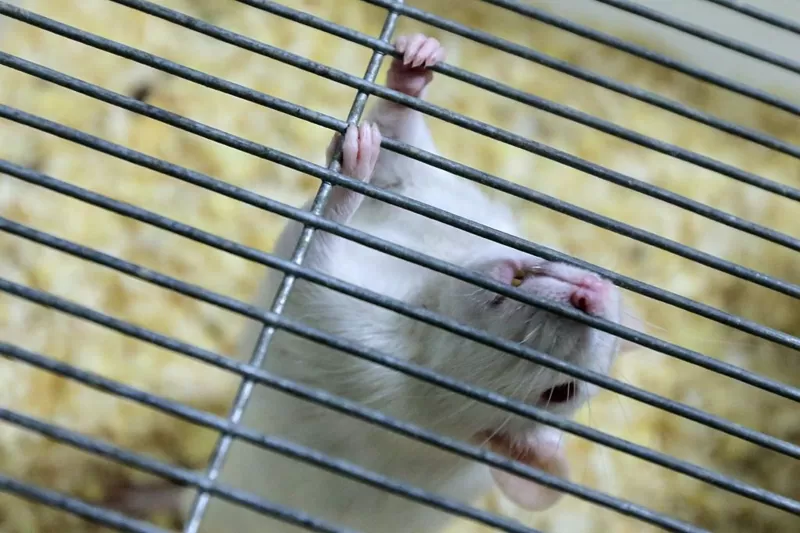
\includegraphics[width=0.44\textwidth]{img/mouse.png}
    \end{center}
    \caption{Процесс закупок трансгенных мышей из-за границы не был очевиден ни сотрудникам лаборатории, ни руководству университета.}
\end{wrapfigure}
"Мы покупаем сравнительно дорогостоящее оборудование, но во время ливней или таяния снега на него начинает течь вода, потому что университет годами не может нормально залатать крышу. Оснащение образовательных лабораторий, где студенты проходят практикум, несравнимо с западными", - поделился на условиях анонимности сотрудник крупной московской лаборатории.

Одни лаборатории, созданные на деньги мегагрантов, успешно существуют до сих пор, а некоторые, даже после полного оснащения, закрываются без дальнейшей финансовой поддержки.

В 2011 году нейробиолог Виктория Коржова закончила Санкт-Петербургский государственный университет и работала в лаборатории, которая тоже создавалась на деньги мегагранта.


"С одной стороны, очень хорошее финансирование, а с другой - денег недостаточно. Все время, которое грант действовал, ушло на организацию самой лаборатории, ремонт помещений и закупку оборудования", - рассказывает Коржова.

Но для исследовательской работы не всегда достаточно просто оборудовать рабочие места.

В лаборатории, где работала Коржова, например, должны были проводиться эксперименты на трансгенных мышах. "Большинство трансгенных мышей производит одна международная компания, которая поставляет их в лаборатории по всему миру, - рассказывает она. - Наш заведующий лабораторией, у которого были деньги на закупку, не знал, как именно привезти мышей в Россию, каков легальный процесс. Университет тоже не мог ему помочь. В какой-то момент мы уже, не совсем шутя, обсуждали, сможем ли мы привезти их в кармане, что совершенно безумная идея".

Проблема решалась почти два года. Все это время ученые были вынуждены придумывать компромиссные варианты, чтобы, как они говорят, получилось что-то похожее на первоначальную задумку.

Одна из важных проблем в России, которая давно решена в странах, где активно развивается наука, - это отсутствие таможенных льгот для научных закупок, считает нейробиолог.

% Сочинский округ Колумбия: почему центр "Сириус" станет федеральной территориейВ отдельных регионах или, вернее, федеральных территориях, эта проблема решена: например, в конце прошлого года в России приняли законопроект о статусе сочинского "Сириуса": компании и люди, которые будут работать на этой территории, получат субсидии на уплату таможенных пошлин.

В других лабораториях страны ситуация иная.

"Нет такой страны, которая бы производила все нужные реактивы для ученых. Нормально, что некоторые реактивы покупаются в США или Европе. При этом везде есть способ быстро получить доставку, - рассказывает Коржова. - Работая в Германии, я могла заказать антитела и получить их максимум в течение недели, а обычно - за два-три дня".

В России же, по ее словам, люди ждут месяцами.

"Антитела - очень чувствительные вещества, которые нужно обязательно хранить в холоде. А если процесс на таможне затягивается, то неизвестно, как они хранятся. Из-за этого еще и эксперименты нужно планировать на год вперед, что не очень реалистично. Приходится идти на компромиссы: я делаю не так, как мне хотелось бы сделать в идеале, а существую в рамках больших ограничений", - говорит нейробиолог.

\subsection{Возвращаются единицы}

Российский кристаллограф, член Европейской академии наук Артем Оганов уехал из России в 1997 году.

Он так вспоминает об этом: "Когда я уезжал, это был 1998 год, зарплаты были, ну я не знаю, пятьдесят долларов в месяц. Это нереально было для существования. Доктора наук продавали стиральный порошок на улице. Я решил уехать. Сейчас времена изменились".


В конце 2014 года Оганов, работавший в США, отказался от гринкарты и вернулся в Россию. "Если при прочих равных выбор: жить у себя дома или не у себя дома (вот я могу здесь заниматься передовой наукой и здесь, я могу и здесь иметь нормальный уровень жизни, и здесь), так вот выбирать нужно всегда свой дом", - объяснял он.

"Таких, кто полностью вернулся в Россию, прервав основные контракты за рубежом, единицы. Подавляющее большинство наших соотечественников, которые успешно работают за рубежом, свои позиции в научно-образовательных организациях развитых стран не оставляют, - говорит Сергей Ерофеев, работающий в американском университете Ратгерс. - Они прекрасно понимают, что это их основная жизнь. Если есть возможность успешно работать с коллегами в России, получать какие-то новые возможности для исследований - они иногда ухватываются за эту возможность".

Многие действительно стараются сохранять и использовать профессиональные связи в России.

\begin{wrapfigure}{l}{0.5\textwidth}
    \begin{center}
        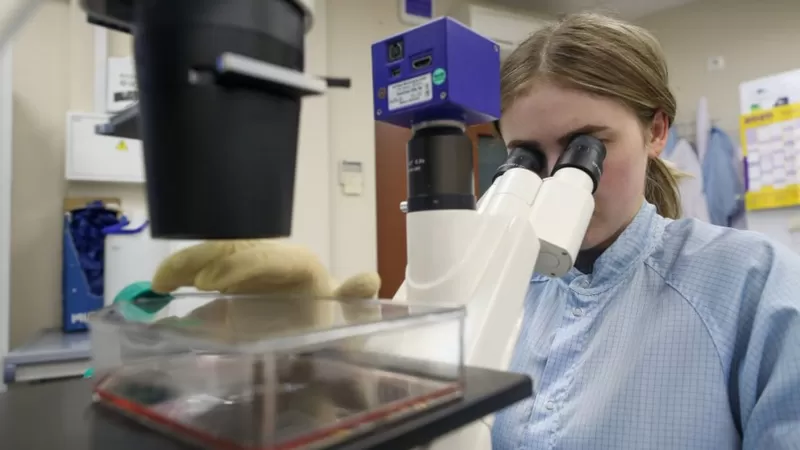
\includegraphics[width=0.48\textwidth]{img/microscope.png}
    \end{center}
    \caption{В России ученым не хватает свободы, считают некоторые уехавшие за границу.}
\end{wrapfigure}
Директор Центра нелинейной физики в Австралийском университете Юрий Кившарь был одним из первых получателей мегагранта. "Мы создали лабораторию - там было человек пять, потом она выросла в центр. Начали набирать новых людей, стало человек сорок. А потом центр стал кафедрой, а кафедра - факультетом. Так появился Новый физтех - физико-технический факультет университета ИТМО", -рассказывает Кившарь.

Сам ученый уехал в Австралию еще из СССР, но связи с российскими коллегами сохранил.

"Когда мы уезжали, это было другое время, - уверен он. - Многие толковые ребята уезжали, лишь бы уехать. Это был отъезд если не насовсем, то надолго. Сейчас у меня есть студенты из Москвы, и в основном они говорят, что уехали на время. Они не собираются оставаться. Сейчас вообще появилось больше возможностей поехать куда-то. В том же ИТМО молодежь посылают за границу на стажировку на год-два, но многие возвращаются", - говорит Кившарь.

\subsection{Национальная идентичность и воздух свободы}

Аспирант астрофизического факультета Принстонского университета США Айк Акопян, до этого работавший на кафедре физики и астрофизики МФТИ, вспоминает, как российские друзья прислали ему ссылку на статью с заголовком: "Американские ученые [далее шли типичные российские имена и фамилии] открыли…"

"Все трое, естественно, работали в США. Вообще сравнивать объем американской и российской науки невозможно, - рассказывает Акопян. - Здесь к науке относятся как к части культуры, как к национальной идентичности. Из-за этого есть частное финансирование науки - то, чего практически нигде в мире нет".


Акопян согласен, что в последние годы ситуация с финансированием науки в России начала улучшаться: "Я учился в России с 2010 года и уехал в 2016-м. За это время ситуация поменялась в лучшую сторону. Многие ученые начали получать огромное количество денег. Но финансы - не основная проблема".

Развития карьеры вне США, где в сфере астрофизики гранты на исследование выдает в том числе и NASA, Акопян не видит. Одним из основных достоинств он считает постоянное взаимодействие ученых.

"Когда открыли гравитационные волны, на следующий же день у нас была информация из первых рук: приехали ученые, которые рассказывали обо всех деталях открытия. Нам не приходится ждать всяких пресс-релизов, все становится открытым, ведется обсуждение. Когда миссия "Кассини" давала результаты - мы опять же всё узнавали от тех, кто занимался проектом".

Другой научный сотрудник университета США, переехавший за границу после окончания МФТИ, соглашается, что для нормальной работы ученых необходимо сочетание независимости и включенности в деятельность научного сообщества:

\begin{wrapfigure}{l}{0.5\textwidth}
    \begin{center}
        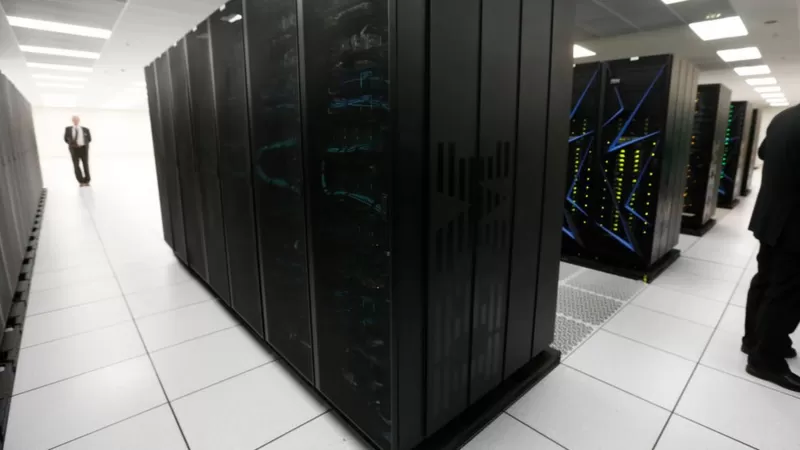
\includegraphics[width=0.48\textwidth]{img/supercomputer.png}
    \end{center}
    \caption{Российские ученые, уехавшие работать в США, считают, что возможностей для развития карьеры здесь больше, а научным сотрудникам доступно более современное оборудование. На фото - суперкомпьютер, на пользование которым можно получить отдельный грант.}
\end{wrapfigure}
"Первое выражается в стабильной зарплате и возможности выбирать направления работы в широких рамках. Второе - в доступности участия в конференциях, семинарах, командировках. До сих пор один из важнейших критериев оценки ученых в Европе и США - это их репутация в международном научном сообществе. Обычно это дает гораздо более точное представление, чем формальные показатели".

"Самое главное, чего не хватает отечественным ученым, - воздуха. Того, что называется научной свободой. Страх сейчас проникает во все поры научного тела", - считает профессор Сергей Ерофеев.

С одной стороны, говорит он, руководство считает, что надо добиваться конкурентоспособности российской науки. Но есть и другая рука, которая главной своей задачей считает контроль.

"А контроль над обществом не предполагает свободы - даже научного мнения", - убежден ученый.

В 2018 году наука в России была официально объявлена национальным проектом. Нацпроект был разработан по следам майских указов Владимира Путина. Было обещано, что к 2024 году Россия должна войти в пятерку ведущих стран, осуществляющих научные исследования и разработки в областях, определяемых приоритетами научно-технологического развития.

Чиновники по-прежнему обещают создать привлекательные условия для работы ведущих российских и зарубежных ученых, а также увеличить финансирование научных проектов и разработок.